\begin{frame}[t,label=mohn]{Mohngewächse - Morphin Alkaloide - Isochinoilin Alkaloide }
  \begin{itemize}
    \item \textbf{Opium} wird als Rohopium aus den unreifen Fruchtkapseln des
      Schlafmohns und verwandter Arten gewonnen
    \item In unter anderem Gehirn und Rückenmark binden sie an Rezeptoren für
      \textbf{Endomorphine}
    \item schmerzlindernd, euphorisierende Wirkung
  \end{itemize}
  \begin{columns}[onlytextwidth,t]
    \begin{column}{0.6\textwidth}
      \begin{minipage}[c][0.9\textheight][l]{\linewidth}
        \begin{figure}
          \textbf{\tiny Papaver Somniferum}\par\medskip
        \includegraphics[height=3cm]{data/mohn/saft}% Place your graphic here
        \end{figure}
      \end{minipage}
   \end{column}
    \begin{column}{0.4\textwidth}
      \begin{minipage}[c][0.9\textheight][l]{\linewidth}
        \begin{figure}
          \textbf{\tiny Morphin}\par\medskip
        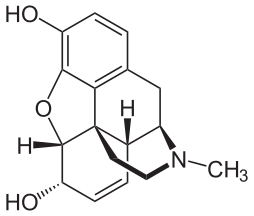
\includegraphics[height=3cm]{data/mohn/morphine}% Place your graphic here
        \end{figure}
      \end{minipage}
    \end{column}
  \end{columns}
  \end{frame}

  \begin{frame}[t]{Morphin-Alkaloide}
    \begin{itemize}
      \item Sie werden aus jeweils zwei Einheiten Tyrosin gebildet
    \end{itemize}

\begin{figure}

    \begin{tikzpicture}
      \node[label=Thebain] (thebain) at (-.5,0)[scale=0.2,draw=none]{
        \includegraphics{data/mohn/thebain}
      };
    \node[label=Codein] (codein) at (3,0)[scale=0.23,draw=none]{
        \includegraphics{data/mohn/codein}
      };
    \node[label=Morphin] (morphin) at (6.5,0)[scale=0.2,draw=none]{
        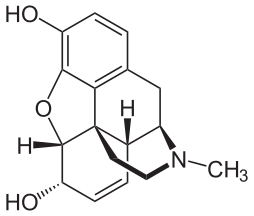
\includegraphics{data/mohn/morphine}
      };
    \draw [{Stealth}-{Stealth}] (thebain) -- (codein);
    \draw [{Stealth}-{Stealth}] (codein) -- (morphin);
    %\node [draw=red] (A) at (0,0) {1};
    %\node [draw=red] (B) at (2,0) {2};
  \end{tikzpicture}
\end{figure}


  \end{frame}

  \begin{frame}[t,label=schoellkraut]{Mohngewächse - Schöllkraut - Spartein }
    \begin{columns}[onlytextwidth,t]
      \begin{column}{0.6\textwidth}
        \begin{minipage}[c][0.9\textheight][l]{\linewidth}
          \begin{figure}
            \textbf{Schöllkraut}\par\medskip
            \includegraphics[height=3cm]{data/mohn/schoellkraut}% Place your graphic here
          \end{figure} 
        \end{minipage}
      \end{column}
      \begin{column}{0.4\textwidth}
        \begin{minipage}[c][0.9\textheight][l]{\linewidth}
          \begin{figure}
            \textbf{Spartein}\par\medskip
            \includegraphics[height=3cm]{data/mohn/sparteine}% Place your graphic here
          \end{figure} 
        \end{minipage}
      \end{column}
    \end{columns}
  \end{frame}

